\chapter{Реализация нейро-семантических моделей для задач управления в АСУТП}

\section{Процесс пастеризации}

Для моделирования были реализованы соответствующие модули. Использовался язык С++, операционная система – Windows 7 и Linux.

Рисунок \ref{fig:Pasteurization_modeling_results} показывает результаты моделирования для следующих значений параметров $k = 525$ и $T = 450$ (см. табл. \ref{table:pasterizer_params}), $P = 0.5$, $T_I = 5$ и $T_D = 0.01$, требуемое задание \SI{20}{\celsius}.

\begin{figure}[H]
    \centering
    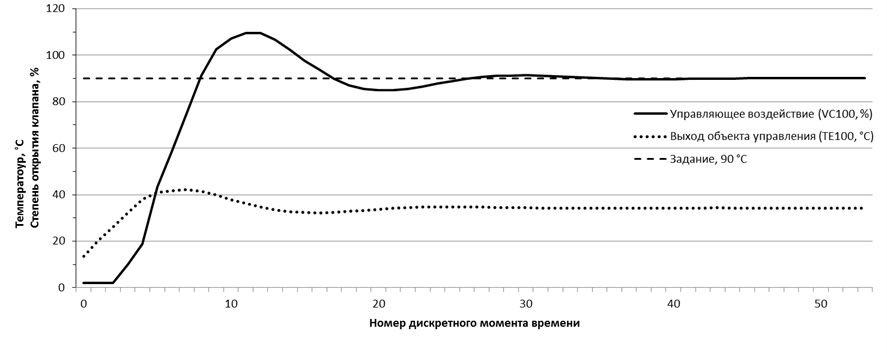
\includegraphics[width=\textwidth]{images/chapter_4/Pasteurization_modeling_results.png}
    \caption{Результаты моделирования процесса пастеризации}
    \label{fig:Pasteurization_modeling_results}
\end{figure}

Для предварительного обучения использовались сохраненные данные работы объекта управления – 50 первых точек c размером окна – 10 (рис. \ref{fig:Pasteurization_modeling_results}), точность обучения 0.00005. Если во время работы в течение 10-ти тактов времени ошибка управления превышала 2, то происходило обучение нейронной сети, точность обучения 0.0001, ограничение на количество итераций обучения – 10.

Результаты моделирования показывают рисунки \ref{fig:Pasteurization_modeling_results_with_typical_PID} и \ref{fig:Pasteurization_modeling_results_with_neuro_PID}.

\begin{figure}[H]
    \centering
    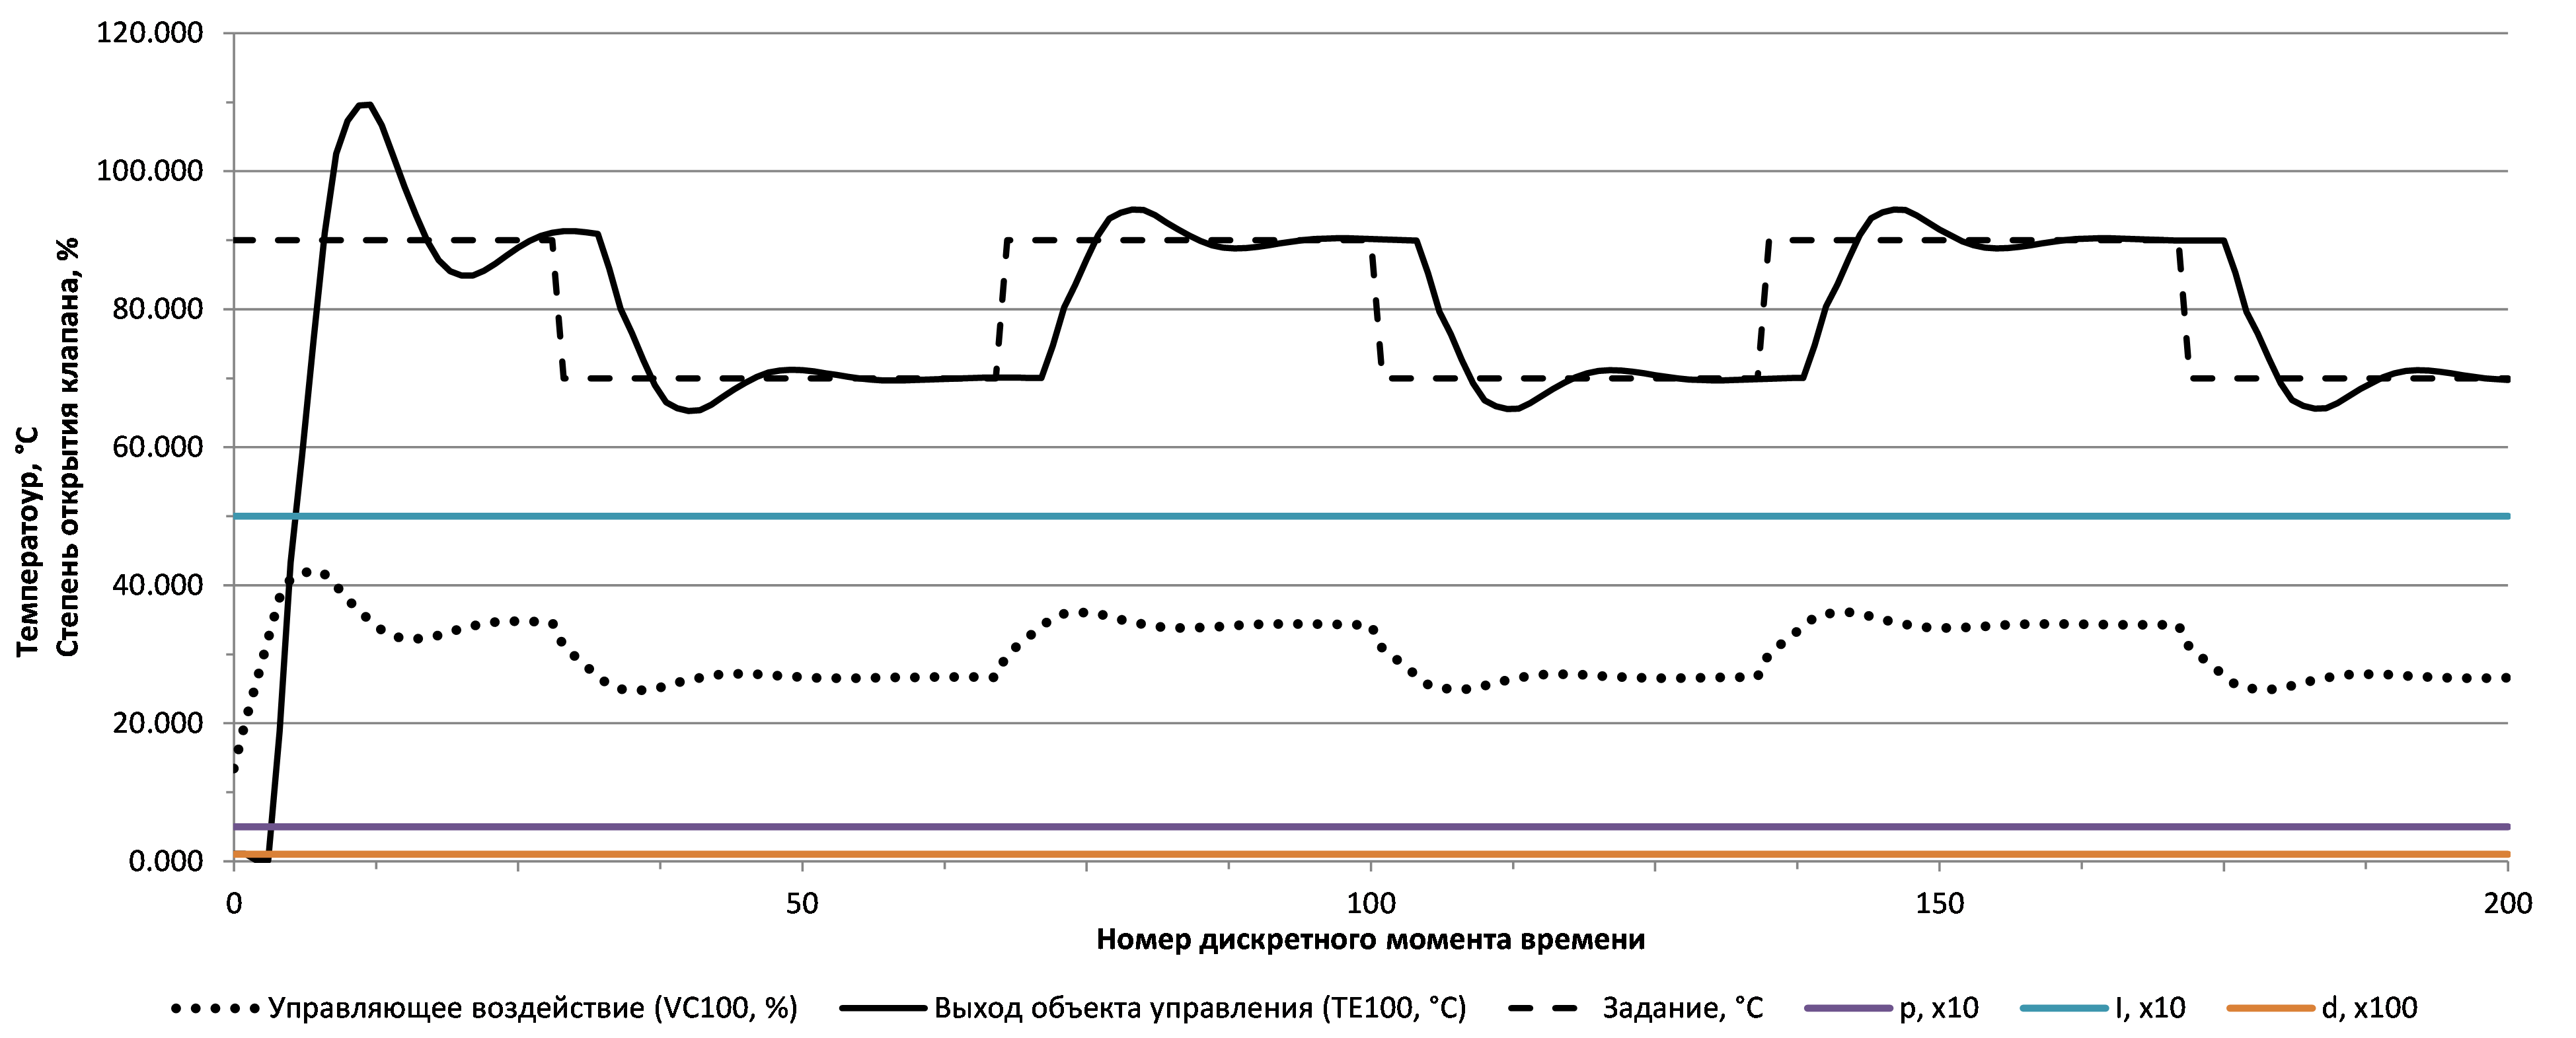
\includegraphics[width=\textwidth]{images/chapter_4/Pasteurization_modeling_results_with_typical_PID.png}
    \caption{Результаты моделирования. Работа обычного ПИД-регулятора}
    \label{fig:Pasteurization_modeling_results_with_typical_PID}
\end{figure}

Видно, что при изменении задания переходной процесс не изменяется и сохраняется один и тот же уровень перерегулирования, так как коэффициенты ПИД-регулятора статичны. Значение перерегулирования $\delta = \SI{5}{\celsius}$ (5\%).

\begin{figure}[H]
    \centering
    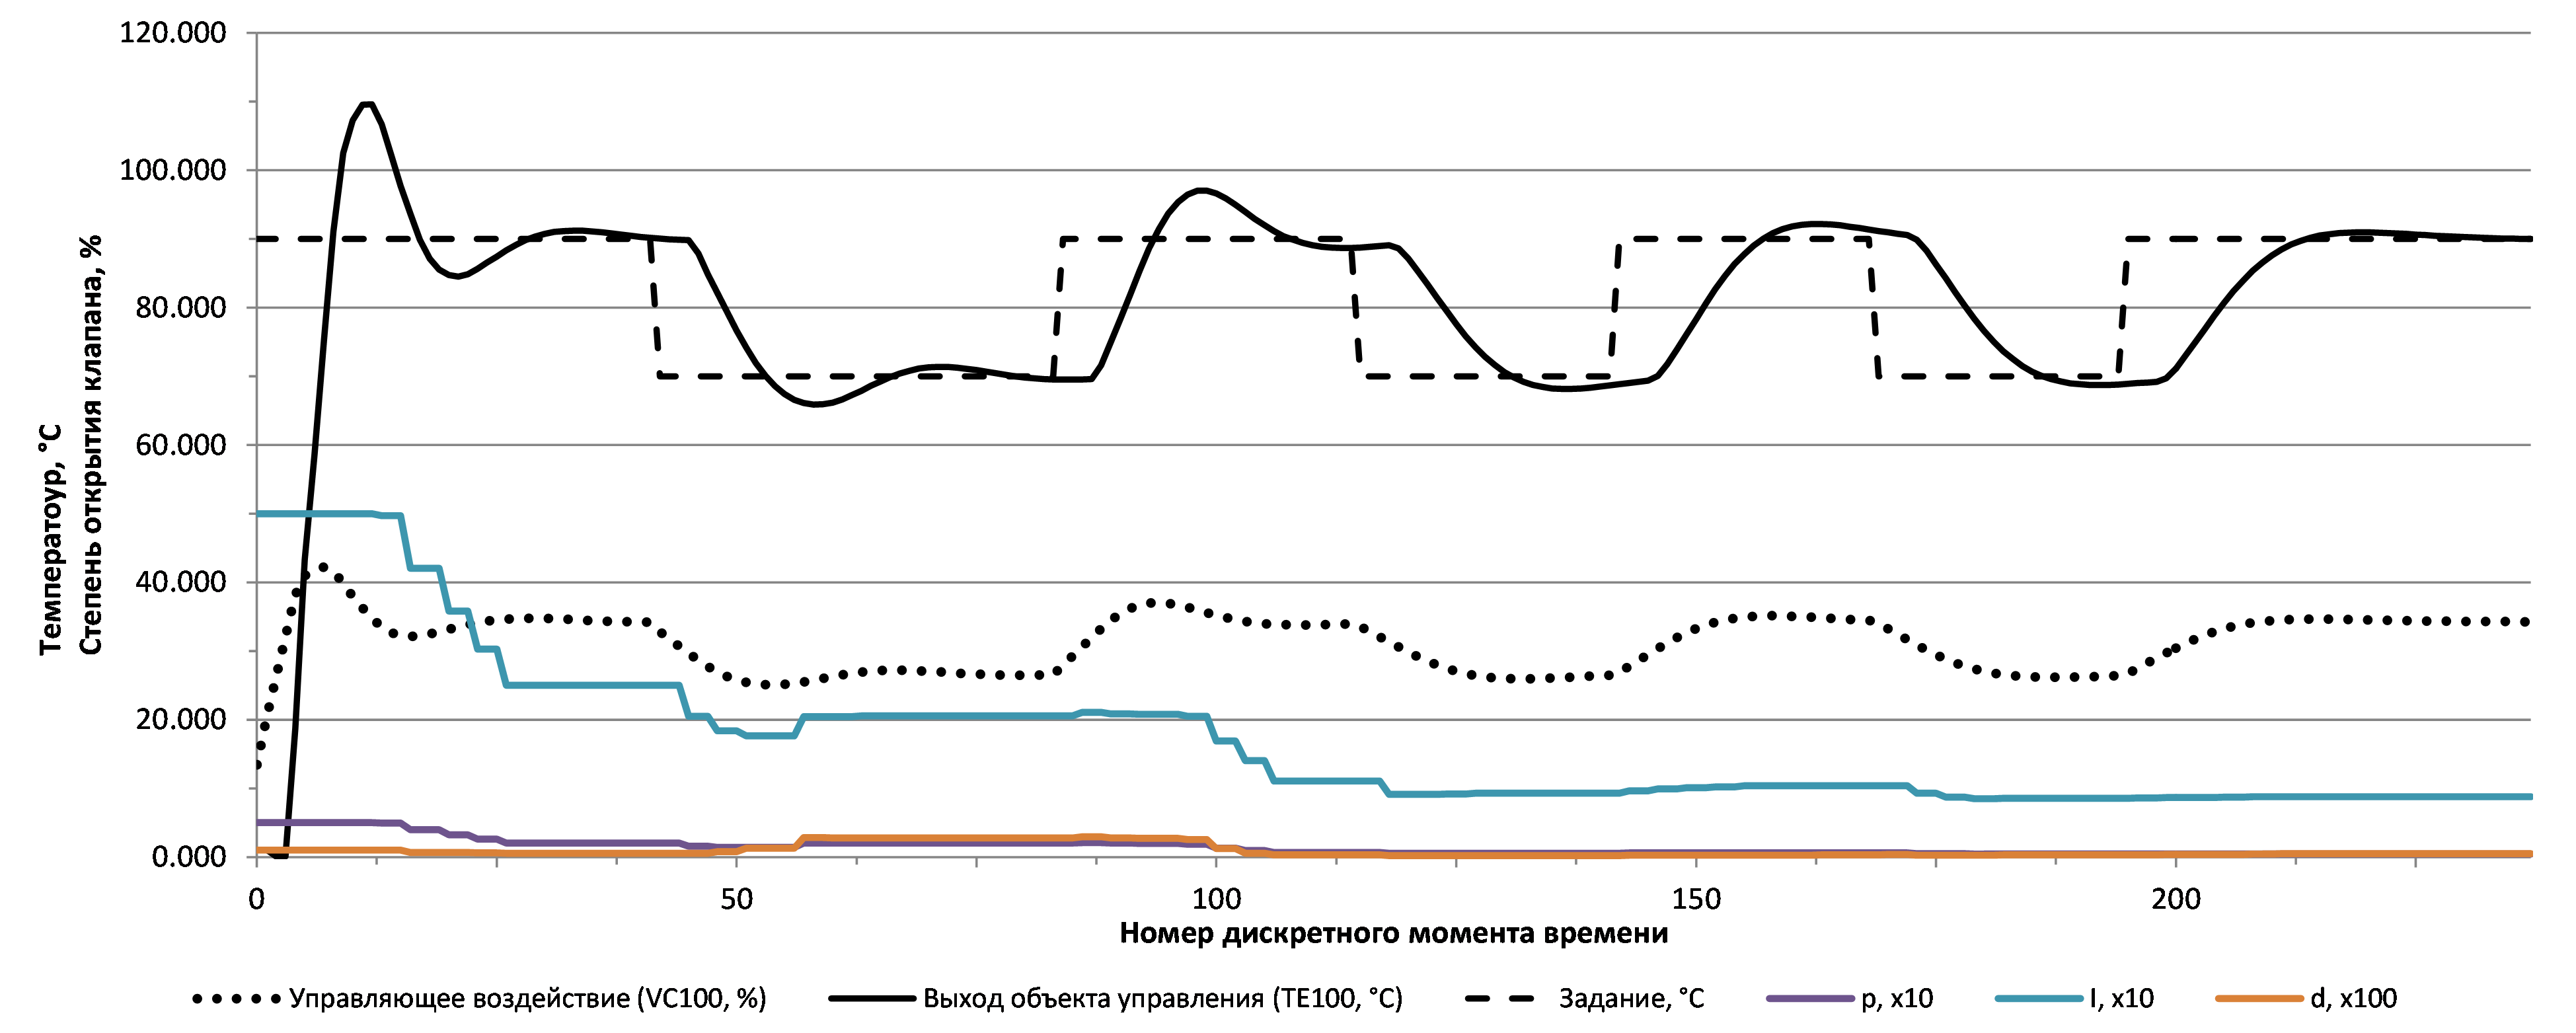
\includegraphics[width=\textwidth]{images/chapter_4/Pasteurization_modeling_results_with_neuro_PID.png}
    \caption{Результаты моделирования. Работа нейро-ПИД-регулятора}
    \label{fig:Pasteurization_modeling_results_with_neuro_PID}
\end{figure}

Можно убедиться, что при четвертом и пятом изменении задания переходной процесс улучшается. Начальные значения коэффициентов - $P = 0.5$, $T_I = 5$ и $T_D = 0.01$, после надстройки – $P = 0.43$, $T_I = 0.9$ и $T_D = 0.005$, значение перерегулирования $\delta = \SI{1}{\celsius}$ (1\%).

В результате была получена следующая модель (структурная спецификация на языке SCn), которая приведена на рисунке \ref{fig:s88_physical_result_ontology}.

\begin{figure}[H]
    \centering
    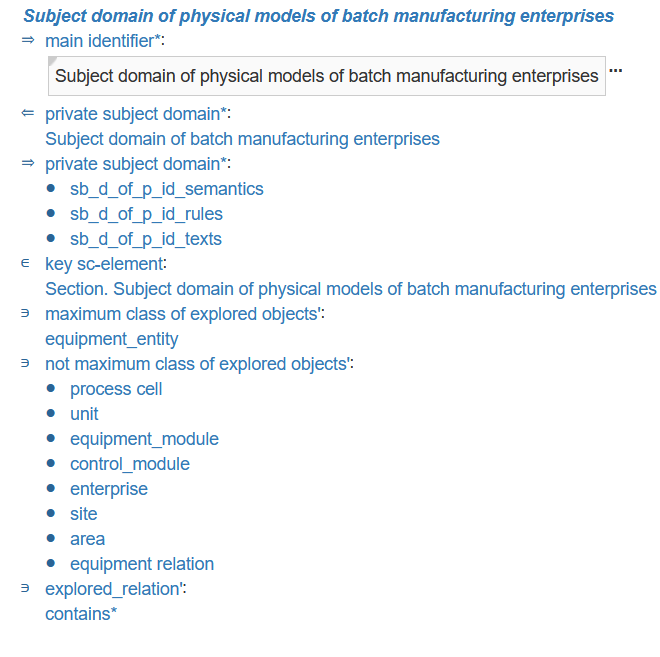
\includegraphics[width=\textwidth]{images/chapter_4/s88_physical_result_ontology.png}
    \caption{Структурная спецификация на языке SCn для физической модели S88}
    \label{fig:s88_physical_result_ontology}
\end{figure}

ПИД-регулятор находится на нижнем уровне - блок управления (equipment module).

Также на рисунке \ref{fig:s88_control_modules} приведена диаграмма классов для EPLANner (проектирование инженером по автоматизации систем АСУТП), также отдельно выделен зеленым ПИД-регулятор.

\begin{figure}[H]
    \centering
    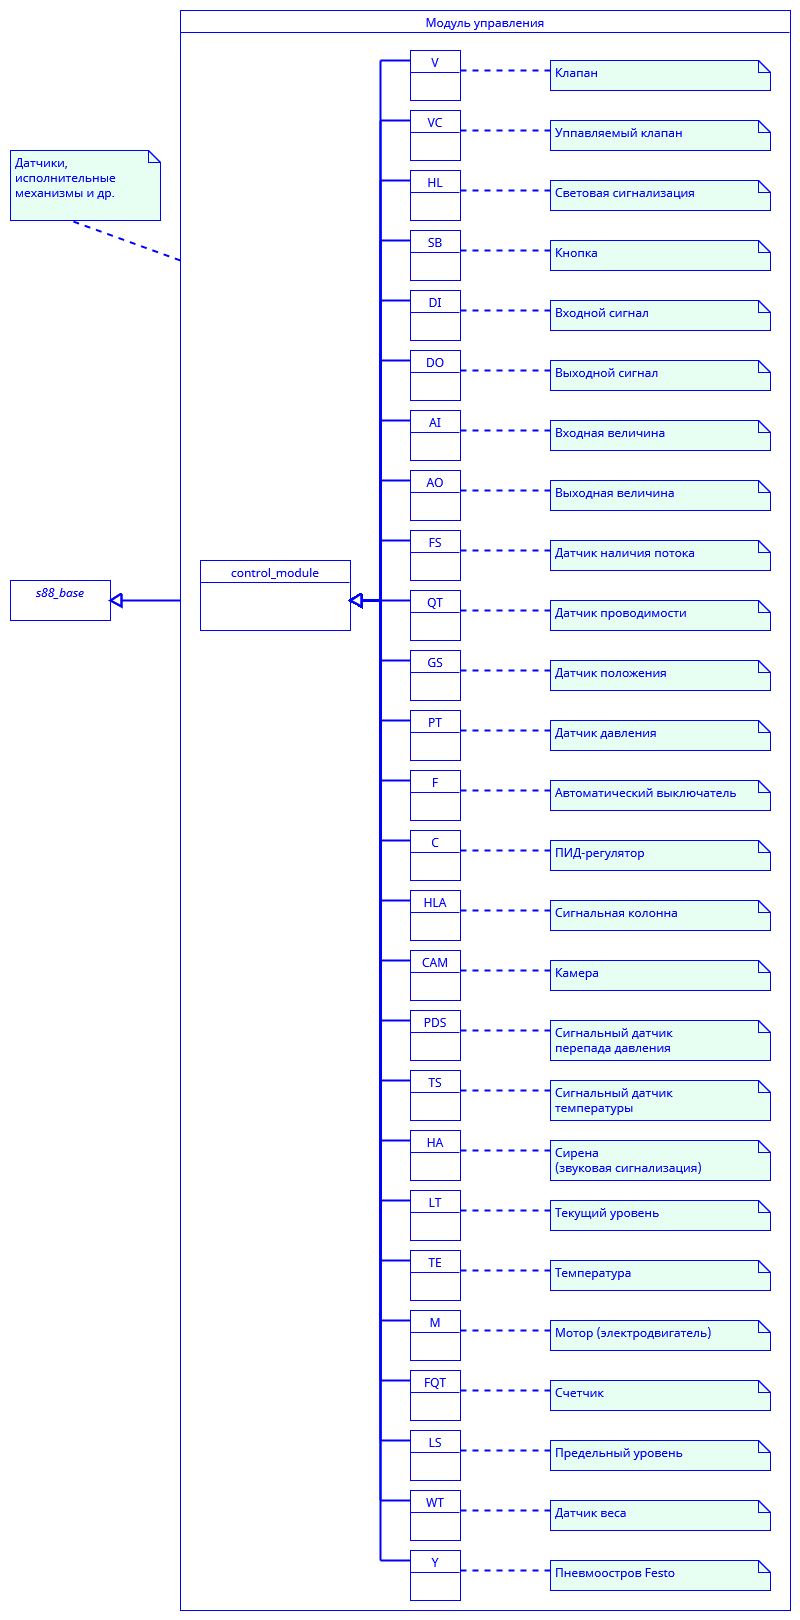
\includegraphics[height=0.9\textheight]{images/chapter_4/s88_control_modules.png}
    \caption{Диаграмма классов для EPLANner для физической модели S88}
    \label{fig:s88_control_modules}
\end{figure}

Разработан агент, который может обращаться к системе управления и получать статус соответствующего блока управления (нейро-контроллера) и получать его состояние для отображения на верхнем уровне (например, для отображения помощи по запросу инженера КиПиА). Также разработан агент, который на основании аварий в соседних проектах может также управлять данным блоком управления (например, через постановки соответствующей операции в паузу). Данное взаимодействие схематически отображено на рисунке \ref{fig:OSTIS_in_control}.

\begin{figure}[H]
    \centering
    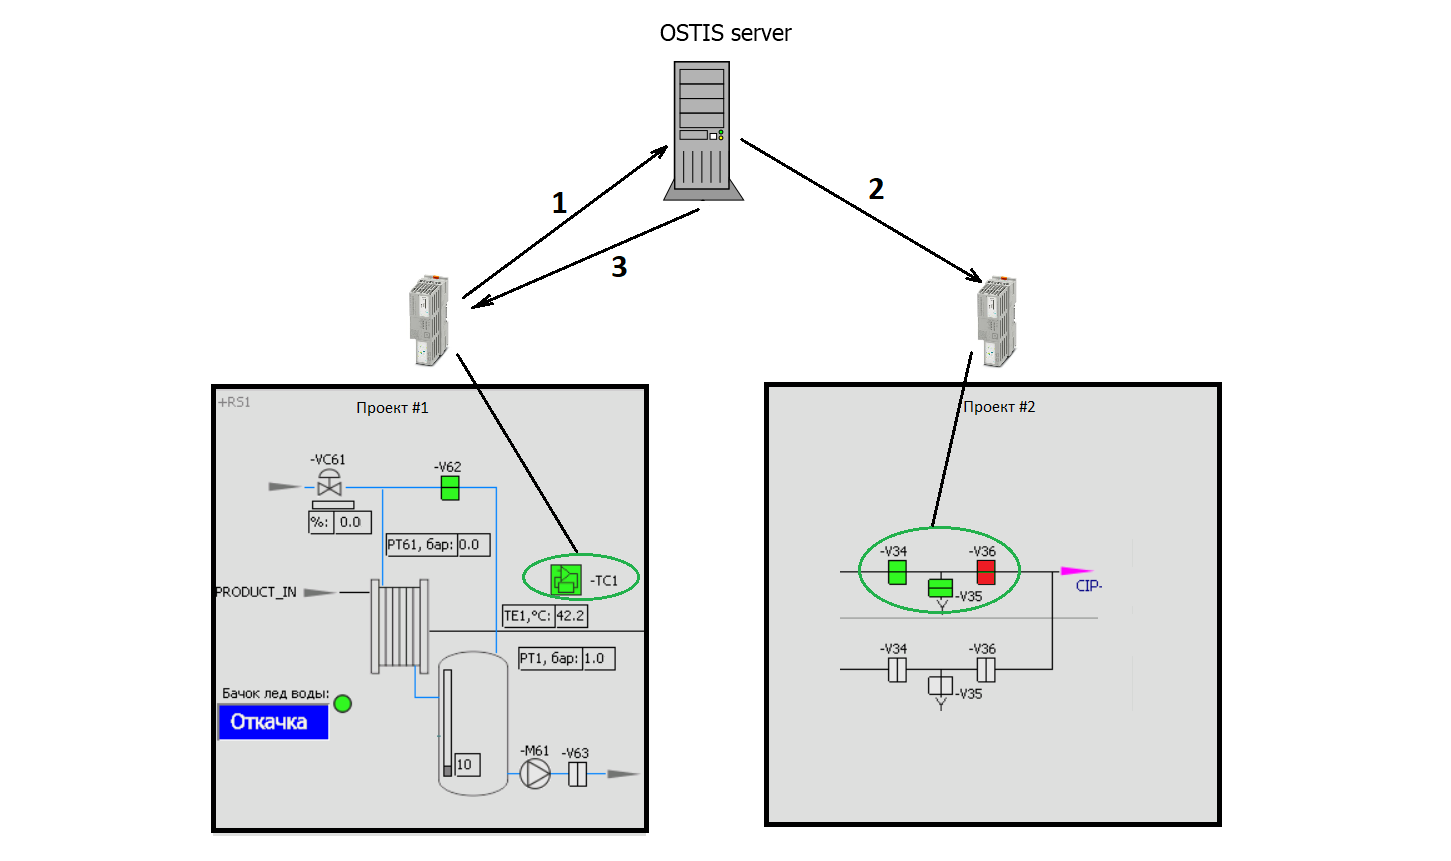
\includegraphics[width=0.9\textwidth]{images/chapter_4/OSTIS_in_control.png}
    \caption{OSTIS-система в управлении}
    \label{fig:OSTIS_in_control}
\end{figure}
